\chapter{Design Evaluation Experiment}

\section{Introduction}

After investigating the technical approach and the benefit to including the passive haptics layer, we seek to investigate the use of the Rapidly Reconfigurable Research Cockpit in a more realistic design evaluation study.
The advantages of using the R3C system would not be useful if it masked defects in a design study.

\section{Methods}

In order to perform a design evaluation study, it was first needed to have a task that the subjects would be doing using the designs.

\subsection{Simulator Setup}

The simulator workstation as configured for each group is \tinytodo{this is not done yet}shown and annotated in Figure \ref{fig:de_sim_groups}.
It was our goal to have as much as possible to be the same between the two configurations.
The joystick and instrument were positioned in the same location for each group.
Neither group had out the window visuals, relying only on the attitude indicator on the instrument.
For the Virtual Reality (VR) group, the visuals showed a plain interior of a cockpit, but the out the window view was black.
Both groups had an aural indication (a click noise of a button being pressed) when a button was activated on the instrument, using the speakers mounted behind the instrument panel.

The main difference between the two groups, beyond the VR group wearing a virtual reality headset, \tinytodo{terrible sentence} was the way the instrument was interacted with.
The VR group used the hand tracker activated system previously described in Chapter \ref{todo fixme}.
For this experiment, the buttons were configured to highlight a blue color when the hand tracker registered a finger within the zone \tinytodo{Find the size of the zone}.
After the 150 msec delay when the button was activated, the highlight would disappear and the button in the virtual world would move inwards as if it were being pushed in (of course, the physical button could not and did not move).
It is also at this time that the press sound would play, as well as any response on the instrument associated with pressing that button.
When the finger left the zone after a successful press, a seperate release sound would play and the button would move back to its starting position.

The Touchscreen (TS) group used a 10.1 inch capacitive touch screen with resolution of 1024x768.
The two instruments were drawn in a web browser, using standard HTML elements for the buttons.
Javascript press and release events were used to simulate the same behavior as described for the VR group, except for the highlighting before a button press.
The visuals of the tracker were rendered on top of the browser window with the same OpenGL rendering code used for the VR group.

%Waveshare 11280

\subsection{Task Design}

With this simulator setup base and the goals of the study, a number of requirements were created to design the task that the subjects would perform.

\begin{itemize}
    \item Flight task using a standard joystick
    \item Second task that requires use of multiple buttons on the instrument
    \item Able to develop simulator for both touchscreen and R3C setup \tinytodo{could explain what this limits}
    \item Able to design two different layouts with one design having distinct flaws
    \item Simple design yet complex enough task to have sufficient workload
    \item Operationally relevant, or analogous to tasks required in a cockpit
\end{itemize}

Ultimately, we designed a task that required number and letter inputs using the buttons, while simultaneously flying a pitch disturbance profile.

\subsubsection{Tracking Task}

The tracking task display was a standard attitude indicator display, shown in Figure \ref{fig:de_ai_display}.
Each tick corresponds to 1 degree in the dynamics simulation, with the major ticks at intervals of 5 degrees.
The attitude indicator was X.X inches square on the instrument. \tinytodo{Thats not a real dimension}

\begin{figure}
    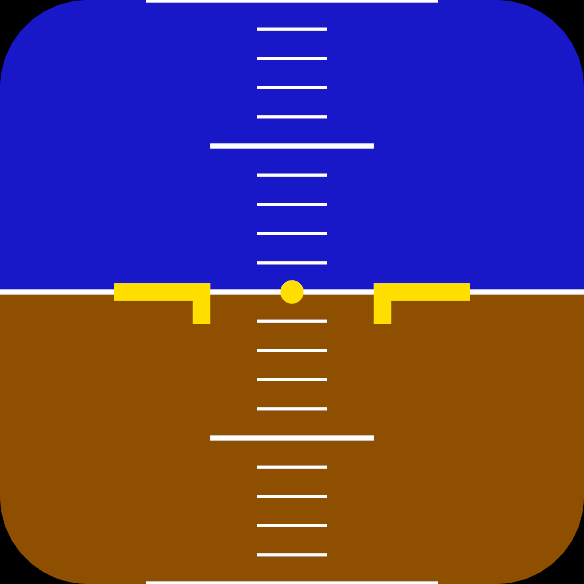
\includegraphics[width=\textwidth]{ai_display.png}
    \caption{Attitude Indicator Display}
    \label{fig:de_ai_display}
\end{figure}

Subjects controlled the one-dimensional (pitch only) task using a joystick with their left hand.
The joystick is pictured in Figure \ref{fig:de_ts_setup}.

The flight dynamics model of the simulator was a stability derivative based model for a Boeing 747 in a low altitude landing configuration.
\tinytodo{Include all the info on the FDM}
The dynamics model was updated and recorded at a rate of 125Hz.

\begin{figure}
    \tikzstyle{block} = [draw, rectangle, minimum height=3em, minimum width=6em]
    \tikzstyle{smallblock} = [draw, rectangle, minimum height=3em, minimum width=3em]
    \tikzstyle{sum} = [draw, circle, node distance=1cm]
    \tikzstyle{input} = [coordinate]
    \tikzstyle{output} = [coordinate]
    \begin{tikzpicture}[auto, node distance=2cm,>=latex']
        \ssp
        \node[input, name=input] {};
        \node[smallblock, right=of input] (K) {$10$};
        \node[sum, right=of K] (sum) {};
        \node[block, node distance=1.5cm, above=of sum] (disturbance) {Disturbance};
        \node[block, right=of sum, text width=5em, align=center] (aircraft) {Aircraft Dynamics};
        \node [output, right=of aircraft] (output) {};

        \draw [draw,->] (input) -- node {$r_{js}$} (K);
        \draw [->] (K) -- (sum);
        \draw [->] (disturbance) -- node {$\theta_D$} (sum);
        \draw [->] (sum) -- node {$\theta_{el}$} (aircraft);
        \draw [->] (aircraft) -- node {$\theta$} (output);
    \end{tikzpicture}
    \caption{Tracking Task Dynamics Block Diagram}
    \label{fig:de_block_diagram}
\end{figure}

The output of the joystick, $r_{js}$, varies from $-1.0$ to $1.0$, and the gain of $10^{\circ}$ was chosen to ensure the pilot had enough control authority to complete the task.

The transfer function of the aircraft dynamics is given as:
\begin{align}
    \mathclap{ % This ignores align for this equation
        \frac{\theta}{\theta_{el}}
        =
        \frac{
            -0.572 (s+0.553) (s+0.0396)
        }{
            (s^2 + 2\zeta_1 \omega_1 + {\omega_1}^2)
            (s^2 + 2\zeta_2 \omega_2 + {\omega_2}^2)
        }
    }\\
    \omega_1 &= 0.0578 & \zeta_1 &= 0.0160 \nonumber \\
    \omega_2 &= 1.12 & \zeta_2 &= 0.798 \nonumber
\end{align}

The disturbance model is based off the model developed in SweetRef.
It is designed to provide a broad spectrum of frequencies that the human controller needs to respond to.

\begin{align}
    \theta_D = K\sum\limits_{i=1}^{12} \left[ a_i \left(\frac{2\pi k_i}{240} \right) \sin\left( \frac{2\pi k_i}{240}t + \phi_i \right) \right]
\end{align}

The $k_i$ terms are given as,
\begin{align*}
    k_1 &= 7, & k_2 &= 11, & k_3 &= 16 \\
    k_4 &= 25, & k_5 &= 38, & k_6 &= 61 \\
    k_7 &= 103, & k_8 &= 131, & k_9 &= 151 \\
    k_{10} &= 181, & k_{11} &= 313, & k_{12} &= 523
\end{align*}
The amplitude terms is $a_i=0.5$ for $i <= 6$ and $a_i=0.005$ otherwise.
The phase terms, $\phi_i$, were randomly selected on the $(-\pi, \pi)$ interval ensuring a uniform distribution.
This random selection was precalculated for each trial, however the order was repeated for each subject so there was no between subjects variance in the disturbance signal.
Furthermore, each subject received the same sequence of disturbance signals for each design, eliminating within subject variance as well.
The disturbance amplitude, $K$, was chosen such that the root-mean square (RMS) of the signal was $3.5$ degrees.

\subsubsection{Prompting Task}

The prompting task was designed to be both a realistic task as well as demanding to create a high workload.
The task would require the subjects to read and memorize a short string of characters and enter it using buttons on the instrument.
To reduce the number of buttons needed, the characters were limited to 1 through 6 and A through F.

The sequencing of the prompts seperated into 10 second ``windows''.
The prompt would appear between 2 and 3 seconds of the start of the window.
From the time of appearance, a seven (7) second timer will start until timeout.
When the subject presses the first button of the prompt, the prompt itself was cleared and asterisk symbols (*) were shown after each button entry by the subject.
After the subject has entered 4 buttons or the timeout occurs, whichever comes first, the prompt or entry so far would clear.
This process is then repeated every 10 seconds.

The prompts themselves were composed of three numbers followed by a letter or three letters followed by a number.
This structure was decided upon to provide a consistent pattern.
The prompts were randomly chosen but were not allowed to have repeat numbers or letters, and for the prompts with three letters, common words or acronyms were filtered out (e.g.\ ``BAD'', ``FDA'').
The selection of letters or numbers as the first three characters was randomly chosen as well.

\subsection{Instrument Designs}

The two different designs used were developed to be both realistic and believable as a cockpit instrument design that would be under consideration, yet still have one design with flaws that would be found in a design evaluation.
We developed a `Keypad' design with the prompting task button keys on the right side and the tracking task on the left, and an `Edgekey' design with the prompt buttons split on either side of the tracking task display.
For both designs the tracking task display was the same size on the display.
The prompting task text is also placed below the tracking task display, and the same font, size and color is used for both designs.
These were kept consistent to limit the number of possible variables between the two designs.

The Keypad design is pictured in Figure \ref{fig:todo}.
The buttons are 1in by 0.75in, with about 0.26in between buttons horizontally and 0.38in vertically.
Each button has the label directly on the top of the button.
For the VR group, the 3D printed instrument had the button labels raised to provide a tactile feedback.
The font was approximately 0.36in in height, and the labels were raised 0.05in.

The Edgekey design is pictured in Figure \ref{fig:todo}.
In this design, there is not a single button for every number and letter.
Instead, the bottom button on either would switch the behavior (and labels) of the remaning six buttons from showing 1 through 6 to showing A through F.
The labels were placed offset from the button on the ``screen'' portion of the instrument, allowing them to change dynamically.
The buttons are slightly smaller in this design, at 0.76in by 0.55in.
The spacing between buttons vertically is the same as the Keypad design at 0.38in.
The center to center distance between the two sides of the button is 7.3in.
For the VR group, the 3D printed instrument had raised nubs on each button covering half the width, 0.08in tall and raised 0.05in.

While some of the more subtle differences were expected to possibly be noted by the evaluation study (e.g.\ having smaller buttons, different position of the flight task), the major flaw we designed into the Edgekey design was the switching key to change from letters to numbers and back.
This additional action fundamentally changed the demands of the task, as the subjects now had to press this additional button to change labels at least once per prompt.
Pressing the switch key was always required between pressing the third and fourth button, and would be required before the first button press if the last state of the buttons did not match the start of the new prompt.
Since there was no gaurentee that the next prompt would start with the instrument on the correct setting, there was an additional cognitive load in determining whether a switch was neccessary at the beginning of the prompting window.

\begin{figure}
    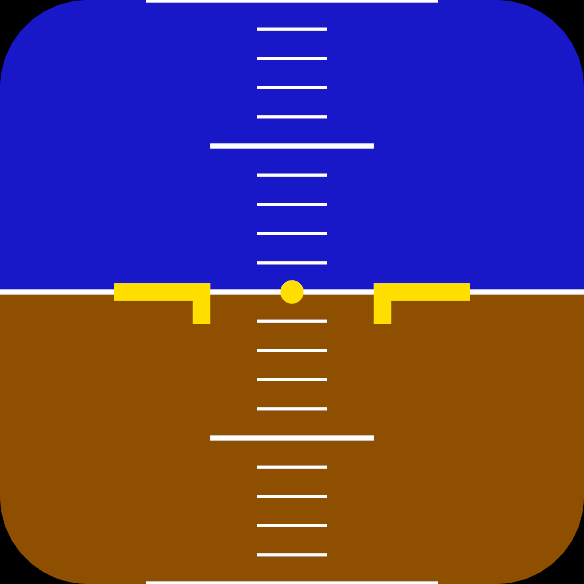
\includegraphics[width=\textwidth]{ai_display.png}
    \caption{Attitude Indicator Display}
    \label{fig:de_ai_display}
\end{figure}

\subsection{Experiment Design}

Subjects were divided into the two groups, TS and VR.
The overall sequence of the experiment started with a training session on the simulator and the task, then an evaluation session for each of the two designs, finally finishing with questionnaires asking about the designs.
The timeline of the experiment was the same for each subject, except for counterbalancing the order that the designs were evaluated.
The training portion started with a slide deck explaining the tasks, the simulator that the subject was using, and the functionality two designs they were to evaluate.
Next, they performed practice trials with just the tracking task and then just the prompting task.
%After basic familiarity with the technology

For the evaluation sessions with each design, they performed six trials with both tasks.
The first three were a minute long, and were considered practice trials, and not included in the data analysis.
The following three were two minutes each, and were the trials used for the results.
Each evaluation session concluded with a two minute trial of just the tracking task.
This was included to investigate if the subject had improved or fatigued at the tracking task.

\subsection{Dependent Measures}

The dependent measures were chosen to evaluate the performance of each task individually as well as the workload of the subject.
For the tracking task, the root-mean square error (RMSE) was calculated for each trial.
The error in this case is simply the pitch shown to the subject, the output of the flight model described above.

The prompting task has two dependent measures, for speed and accuracy.
For speed we consider the \textit{response time}, defined as the time between the prompt is first shown to the subject and when they press the first button of their response entry.
The accuracy is measured by how many prompts they complete correctly.
Twelve prompts are shown to the subject within each trial, and these measures are meaned per trial and then per design for each subject.

For workload, a NASA Task Load Index (TLX) survey was administered after they completed each design.
The TLX survey asks for a rating of their workload between 0-100 for the following subscales: Mental Demand, Physical Demand, Temporal Demand, Performance, Effort, and Frustration.
Our implementation allowed selection of the ratings within increments of 5, and included anchors of "Low" and "High" at the extrema of 0 and 100, respectively (except for Performance, which uses "Good" and "Bad").
The midpoint (50) was also visually indicated with a larger tick.
The ranked pairs modification was used and completed for both times the subject took the survey.
This modification asks the subject, for each of the combinations of pairs of subscales, which of the two they felt contributed more to their workload.
The number of times they select each subscale is used a weight to calculate a weighted mean for the total TLX score.

Finally, the subjects were given a questionnaire asking for their feedback on each instrument design.
For each design, the subjects were asked the following questions:
\begin{itemize}
    \item Please comment on any difficulties you had performing the prompting task with this design especially in contrast to the other design.
    \item Please comment on anything you liked in this design.
    \item Please comment on anything you did not like in this design.
    \item Any other comments?
\end{itemize}
Additionally, the following questions were asked:
\begin{itemize}
    \item Which instrument design did you prefer? Why?
    \item Did you experience any physical fatigue during the experiment? Where?
    \item Any other comments?
\end{itemize}
An open form text box was used for the response field for each of these questions.

In a standard design evaluation study, the feedback received from the users in this questionnaire (and other debriefing interviews) would often be the main source for carrying out re-design.
The goal of this experiment is to determine and document in which ways does this feedback differ.
For example, if most subjects in one group noted issues with the size of a button, while no one in the other group found an issue with that button, this would indicate that using this VR system may not highlight the same issues regarding button sizes.
The groups were purposely left ambiguous in the example, as it does not matter which group found the flaw and which group did not comment on it.
Although we could postulate as to which group are ``correct'', it is not a useful exercise, as the only result is to document what potential differences could arise.

To analyze these results, the sentences from the open form responses were first separated into single feedback comments, and reworded to use common language.
If a subject repeated the same comment in the answers to multiple questions, they were only counted once.
Each of these simplified feedback comments were assigned to a category or overall summary of their feedback.
This process was completed separately for each group.
To summarize the differences, we will look for feedback that is unique to a certain group, as well as the frequency of the comments that are common.

\subsection{Statistical Tests}

The quantitative dependent measures are tested with a two-way ANOVA, with one within subjects factor (Design) and one between subjects factor (Group).
The Design factor contains two levels, the two designs each subject tested, Edgekey and Keypad.
The Group factor also contains two levels, the VR group and the TS group.
When the ANOVA showed significance in the interaction test, post-hoc repeated measured t-tests were undertaken to determine the significance of Design within each Group.
An independent samples t-test was used to test the signifinace of Group within each Design.
All effects were considered statistically significant at the 0.0125 level.
Statistical significance level was corrected using the Bonferroni correction considering the 4 different dependent measures being tested ($\alpha = 0.05/4 = 0.0125$).
Effects which have a signifigance level between $0.05<p<0.0125$ are considered to be marginally significant.

\section{Results}

\subsection{Demographics}

Twenty-three subjects were recruited from the UC Davis engineering undergraduate and graduate student population.
Twelve subjects were placed in the VR group, and the remaining eleven in the TS group.
The mean age was $21.0 (\sigma = 3.14)$, with 19 male and 4 female subjects.
The female subjects were balanced between the two groups.
Most subjects had no flight experience (two were student pilots), and all of the VR group subjects indicated that they had less than one hour of experience using virtual reality headsets.

\subsection{Performance Measures}

\subsubsection{Tracking Task RMSE}

The performance of the tracking task was measured using the root-mean square average (RMSE) of the pitch.
The effect of Group yielded an $F$ ratio of $F(1, 21) = 21.4, p < 0.001$ indicating a significant difference between VR ($M=1.28\mathrm{deg}, \sigma=0.38\mathrm{deg}$) and TS ($M=1.97\mathrm{deg}, \sigma=0.38\mathrm{deg}$).
In both groups, subjects were performing the tracking task using the same joystick.
The most direct factor that could contribute to the decreased performance in the tracking task for the VR group is that the visuals of the tracking are the loss of visual acuity in the tracking.
Indirectly, the additional workload of the prompting task could be taking attention away from the tracking task.
The effect of Design indicated a marginally significant difference ($F(1, 21) = 5.94, p=0.024$) for the tracking task RMSE between Keypad ($M=1.57\mathrm{deg}, \sigma=0.51\mathrm{deg}$) and Edgekey ($M=1.70\mathrm{deg}, \sigma=0.52\mathrm{deg}$).
The only change in the tracking task display between the two instrument designs is the position moves from being on the left side for the Keypad and the middle for the Edgekey.
This suggests that any difference on the tracking task performance between the groups would be related to additional workload from the prompting task.
The interaction effect was not significant ($F(1, 21) = 0.17, p=0.69$).
%No interaction effect indicates that even if the VR group had lower performance, the same factors are likely affecting the difference between the designs

To further investigate the change in performance between the two groups, we can investigate the trials where the subjects were only doing the tracking task.
At the end of each evaluation session, the subjects ran a single trial that was just the tracking task.
These trials were included to be used as a test of the assumption that the subjects were no longer learning, but can also be used as a test of the Group factor on the tracking task performance.
The effect of group on RMSE for the tracking-only trials yielded a marginially significant difference ($F(1, 21) = 4.81, p = 0.039$) between the VR Group ($M=1.32, \sigma=0.50$) and the TS Group ($M=0.91, \sigma=0.43$).
There was no signifigant difference for the effect of design ($F(1,21) = 0.068, p=0.80$).
The interaction effect between group and design was also not significant ($F(1,21) = 3.21, p=0.087$).

Although the tracking only trials found a marginally significant difference for the group, the difference was much more distinct for the trials with both tasks.
This indicates that when the subjects were focused on the single task, they were able to mitigate most of the visual resolution differences between using a touchscreen and the virtual reality screen.
Additionally, the marginally significant difference between the designs for the trials with both tasks was reduced to no signifigance when the second prompting task was removed.
This also points to the additional workload of the prompting task causing a performance drop on the tracking task.
The factors leading to the added workload of the prompting task are investigated in the other performance measures.

\subsubsection{Prompt Response Time}

The first measure of the prompting task is the response time of the subject.
The response time is defined as the time from the prompt is shown to each subject until they press the first button of the prompt.
For the Edgekey design, it would be possible that the subject had to start with the switching button if the new prompt did not start with the same mode (letters or numbers) as the previous prompt.
Since this button would not clear the prompt when it was pressed, it is not considered the first button of their entry.
However, this would still require an additional movement of the subject, adding additional time.
For this reason, the prompts which required the subject to start with the switch key are filtered out of this analysis.

The response time was unique among the dependent measures, as all tests were insignificant.
The effect of group yielded an $F$ ratio of $F(1, 21) = 1.19, p = 0.29$ indicating no significant difference between VR ($M = 2812\mathrm{msec}, \sigma = 383\mathrm{msec}$) and TS ($M = 2594\mathrm{msec}, \sigma = 567\mathrm{msec}$).
One factor that could influence the response time between groups is the additional time to activate a button in the VR environment versus the touchscreen.\tinytodo{explain this?}
However, a large portion of the response time for the subject is their cognitive processing of the prompt -- recognizing the new prompt has appeared, reading it, then memorizing it.
Beyond potentially differences in the visual environment, the cognitive portion should not take more time for one group or the other.
A potential reason that there could be a lower than expected difference between the group means is that some VR subjects learned to keep their hand closer to the instrument so that the hand tracker could keep it in view.
When the hand tracker lost view of the hand, the reacquisition time could be significant, so holding it close to the instrument would prevent this from happening.
This issue comes up again when looking at the subjects' response to questions about fatigue.
The effect of design was also insignificant ($F(1, 21) = 0.68, p = 0.42$) between Keypad ($M=2728\mathrm{msec}, \sigma=512\mathrm{msec}$) and Edgekey ($M=2687, \sigma=471\mathrm{msec}$).
The biggest difference between the two designs is the switching key on the Edgekey design.
As described above, the need for an additional switch press before the first prompt button was filtered out, so we are only comparing prompts where the first button was available right away to the subject.
Since the Edgekey design had more time pressure due to the need for the switch key, subjects could have learned to respond quicker to adapt for this.
However, these differences in the design did not appear to have a significant effect on the response time.
Finally, the interaction effect was not significant ($F(1, 21) = 0.001, p = 0.96$).

\subsubsection{Prompts Correct}

The second measure of the prompting task is the accuracy of the subjects in correctly completing the prompt.
To get the prompt correct includes two important components for the subject.
First, they must remember the prompt as they enter it, and second, they must be able to physically press the buttons within the seven second response window.
For the statistical test we are using hte count of how many prompts each subject completed successfully per trial.
Among the incorrect prompts, we can differentiate between whether the subject entered the prompt incorrectly (failure to remember the prompt) or whether the subject ran out of time (failure to physically press the buttons).
There were 12 prompts per trial, and every subject completed three trials for each design.

The number of correct prompts had a significant interaction effect between group and design ($F(1, 21) = 27.8, p < 0.001$), meaning the main effects must be intrepreted with the post-hoc tests as well.
Both main effects were significant, the effect of group yielded an $F$ ratio of $F(1, 21) = 43.9, p < 0.001$ while the effect of design yielded an $F$ ratio of $F(1, 21) = 64.1, p < 0.001$.

For the effect of design on the VR group, the repeated measured t-test indicated a significant difference ($t(11) = 8.0, p < 0.001$) between the Keypad ($M = 8.11, \sigma = 1.62$) and the Edgekey ($M = 4.00, \sigma = 2.37$)
The TS group had a marginally significant difference ($t(10) = 2.28, p = 0.045$) between Keypad ($M = 9.82, \sigma = 1.38$) and the Edgekey ($M = 10.6, \sigma = 0.96$).\tinytodo{these are backward}
Both groups had trouble with the additional time pressure caused by the Edgekey design requiring the use of the switch key.
The TS group performed a lot closer to their performance in the Keypad design, only getting approximately 1 fewer prompt correct.
The VR group had much more difficulty in the Edgekey design, correctly completing about half as many as they completed in the Keypad design.
However, it appears that they had more difficulty in both designs compared to the TS group.

This agrees with the post-hoc tests for differences in design between groups.
These tests had significant effects for both the Keypad design ($t(21) = 4.44, p < 0.001$) between the VR group and the TS group, and the Edgekey design ($t(21) = 7.05, p < 0.001$) between the VR group and the TS group.
The main effect of group clearly has a meaningful effect, which found the VR group ($M = 6.05, \sigma = 2.88)$) had significantly fewer correct prompts than the TS group ($M = 10.2, \sigma = 1.2$).
This difference is largely due to subjects not being able to complete the prompt.
Figure \ref{fig:de_correct_stacked} shows the breakdown of the mean result of each trial for each group and design.
Across all groups and designs, very few prompts were completed that were incorrect, and most of the differences in number completed correctly is due to the incomplete prompts.
A contributing factor for this would be the method of button activation used for the VR group combined with the time pressure.
Another contribution would be the limitations of the hand tracker.
When the hand tracker lost tracking or gave bad information, it became hard or impossible for the subject to activate a button until the hand tracker returned to normal.
When this happened in the middle of a prompt, the amount of time it took to recover from the bad tracking would lead to a timeout on the prompt entry, causing an incomplete prompt.
The variance of number correct was also much larger in in the VR group, which could be caused by the unfamiliar nature of the VR environment compared to a touchscreen.


\subsubsection{NASA TLX}

After the subject completed their trials on each design, they completed a NASA TLX workload survey.
Their weighted scores are used here as a measure of their self-reported workload.
The interaction effect between group and design was found to be significant ($F(1, 21) = 8.25, p < 0.001$).
The main effects showed a significant differene in design ($F(1, 21) = 23.6, p < 0.001$), but not in group ($F(1, 21) = 1.69, p = 0.21$).
This could mean that the group did not affect the TLX score, but in the presence of an interaction effect, the post-hoc tests will guide the interpetation.

The repeated measures t-tests indicated significance between designs for the VR group ($t(11) = -4.20, p = 0.001$) between the Keypad design ($M = 54.4, \sigma = 20.4$) and the Edgekey ($M = 85.6, \sigma = 11.2$)
There was a marginally significant difference between designs for the TS group ($t(10) = -2.72, p = 0.02$) between the Keypad design ($M = 61.5, \sigma = 4.46$) and the Edgekey ($M = 69.2, \sigma = 10.1$).
The effect of design was much stronger in the VR group, but both groups indicated higher workload on the TLX scores for the Edgekey design.
This follows from experimental design which hypothesized that the Edgekey design would be more difficult.
One factor that could have contributed to a larger difference in scores for the VR group could be the increased difficulty subjects had in completing the prompt, as seen in the results of the number of incorrect and incomplete prompts for the VR group using the Edgekey design.
The effect of group was not shown to be significant in the ANOVA analysis, but the independent samples t-test showed a signifigance for the Edgekey design ($t(21) = 3.69, p < 0.01$) between the VR Group ($M = 85.6, \sigma = 11.2$) and the TS Group ($M = 69.2, \sigma = 10.1$).
With the Keypad design, The effect of group was not significant ($t(21) = -1.13, p=0.27$) between VR ($M = 54.4, \sigma = 20.4$) and TS ($M = 61.5, \sigma = 4.46$).
These tests further illustrate that the VR group found a higher workload for the Edgekey design specifically, as both groups rated the workload in the Keypad design similarly.
%Furthermore, although the VR group did have a larger effect on design, the TS group had a marginally significant effect, indicating that the main effect of design was a meaningful result.

\subsubsection{Summary}

A summary of the signifigance results from the ANOVA and post-hoc t-tests for all the performance measures are shown in Table \ref{tab:de_anova}.
The signifigance is indicated by `$*$' for $p<0.0125$, `+' for $0.0125<p<0.05$, and `-' for no signifigance.
The interaction effect is indicated by the ``Group:Design'' column.
For the measures with significant interaction effect, the post-hoc t-tests are shown per group.

\begin{table}
    \centering
    \includetable{de_anova_summary.tex}
    \caption{Statistical Signifigance Test Results. `$*$' indicates signifigance at the $p<0.0125$ level, `+' indicates marginally significant ($0.0125<p<0.05$), and `-' indicates no signifigance. Group:Design is the interaction effect between Group and Design.}
    \label{tab:de_anova}
\end{table}

\subsection{Design Feedback}

The categories of feedback and the counts of how many times they occured for each group is summarized in Table~\ref{tab:de_feedback}.

\begin{table}
    \centering
    \includetable{de_feedback.tex}
    \caption{Counts of Design Feedback Comments per Group}
    \label{tab:de_feedback}
\end{table}

By far the issue that received the most feedback was the difficulty of using the switch key (Edgekey, Switch Difficult).
Most of the complaints just centered around the extra difficultly of habving to press another button.
Some noted that it took extra time (with no extra time given), it added to the mental demands of the task, it was difficult to see which mode the instrument was in.
Both groups disliked the switch key, and mentioned it just as frequently.
\begin{displayquote}[TS Subject]
    Switching from numbers to letters was hard, especially if I was trying to compensate for turbulence and was struggling at the time.
\end{displayquote}
\begin{displayquote}[VR Subject]
    I did not like how much extra work it was. It took so much extra focus that I forgot I was flying with the joystick
\end{displayquote}

Many subjects noted the familiarity of the Keypad design (Keypad, Familiar) and that having the buttons close together (Keypad, Buttons Proximal) as things they like about that design.
The familiarity was noted more often for the TS Group, but both were some of the more frequent comments within each group.

One comment about the Edgekey design that got more frequent mentions from the TS Group was that they found having the flight task in the middle of the display, centered between the buttons, was preferred (Edgekey, Centered Flight Task Better).
The subjects who noted they preferred the Edgekey design almost uniamonously cited this as their reason for their preference.
The comments that fed into this category also included subjects who noted the difficulty of splitting their focus back and forth with the Keypad design.
Interestingly, two of the TS Group subjects noted that they would have found the Keypad easier if they had tactile feedback to guide their input.
It is possible that the reason the VR Group subjects did not note this as often is because with the tactile feedback they were able to keep visual focus on the left half of the screen in the Keypad design, thus not seeing benefit from the centering of the flight task display.
\begin{displayquote}[TS Subject]
    \textins{The Edgekey design} forced me to pay more attention to what I was typing, this wouldn't have been a problem if the keypad was a physical device that allowed me to locate the numbers and letters without looking, much like the dots on a computer keyboard.
\end{displayquote}
\begin{displayquote}[VR Subject]
    I like that the flight control was centred, so you could see it even when you were looking at the buttons.
\end{displayquote}

The most notable exceptions to providing similar feedback between groups are the categories that relate to fatigue issues.
Many subjects in the TS group noted fatigue cause from using the joystick, yet none in the VR group did, even though they were using the same joystick setup, and sitting in the same location.
The VR group did note more fatigue caused by using their other arm for the prompting task.
This fatigue seemed to be caused by the additional effort needed to have the hand tracker recognize the hand.
For example, one subject wrote:
\begin{displayquote}[VR Subject]
    My right wrist was somewhat fatigued.  Though I think this is mostly from positioning my hand for the simulator to recognize my input.
\end{displayquote}
Some of this additional effort was due to subjects learning to hold their prompting task hand ``hovering'' while waiting for the next prompt.
This was done to keep the hand in view of the hand tracker as when the hand leaves the field of view, the reacquisition will slow down the entry of first button.
Many subjects organically learned this, and kept their arm in front of the instrument.

Similarly to the fatigue issues being different, there were some comments that were due to the technology being used moreso than the designs themselves.
The obvious ones are the subjects who noted difficulty using the hand tracker, but some of the other categories had comments that may have been caused by this.
For example, the keypad design was noted as causing more mistakes for some subjects.
For the TS Group, this was due to the touchscreen being so quick to use:
\begin{displayquote}[TS Subject]
    \textins{S}ince I was able to go more quickly with this layout, I had more mistakes in the entry.
\end{displayquote}
One subject in VR noted a common problem caused by the hand tracker which caused more mistakes in the Keypad design.
When the hand tracker was having registration issues it would sometimes place the other fingers mistakenly in the activation zone of the buttons underneath the one being targeted, causing multiple buttons to be pressed in a short period of time.
\begin{displayquote}[VR Subject]
    There's more unintended register since other fingers might trigger the buttons.
\end{displayquote}
Although only one subject noted this, it was observed happening to many subjects\footnote{For the VR group, eight of the twelve subjects had the wrong button register within 200msec of the last button in the Keypad. In the other designs and groups this happened to only one or two subjects.}.


\section{Discussion}


\subsection{Effects of Training}
% A blind evaluation of the feedback may have been better

% A more extensive interview may have been more standard, not done here due to the subject population
% Also due to the goal of the experiment -- leading questions in the interview could have caused a bias, by leaving it proctor-free and rigid for each subject, it removed such a bias

\section{Conclusion}
